% !TeX spellcheck = en_US
\chapter{Introduction}

\todo{maybe prologue?}

\section{Motivation}

\todo{Motivation}

\section{The IceCube Neutrino Observatory}

Since January 2011, the IceCube Neutrino Observatory at the South Pole is measuring neutrinos emanating from various sources. For this purpose a detector instrumented with digital optical modules (\enquote{DOMs}) is installed deep in the antarctic ice. 5160 of these optical sensors are arranged on 86 strings at a height between \SI{1450}{\meter} and \SI{2450}{\meter} below the surface. The central region of this In-Ice Array which has a higher density of DOMs is called \enquote{DeepCore}. Figure \ref{icecube:detector} shows a sketch of the detector arrangement.

\begin{figure}[h]
	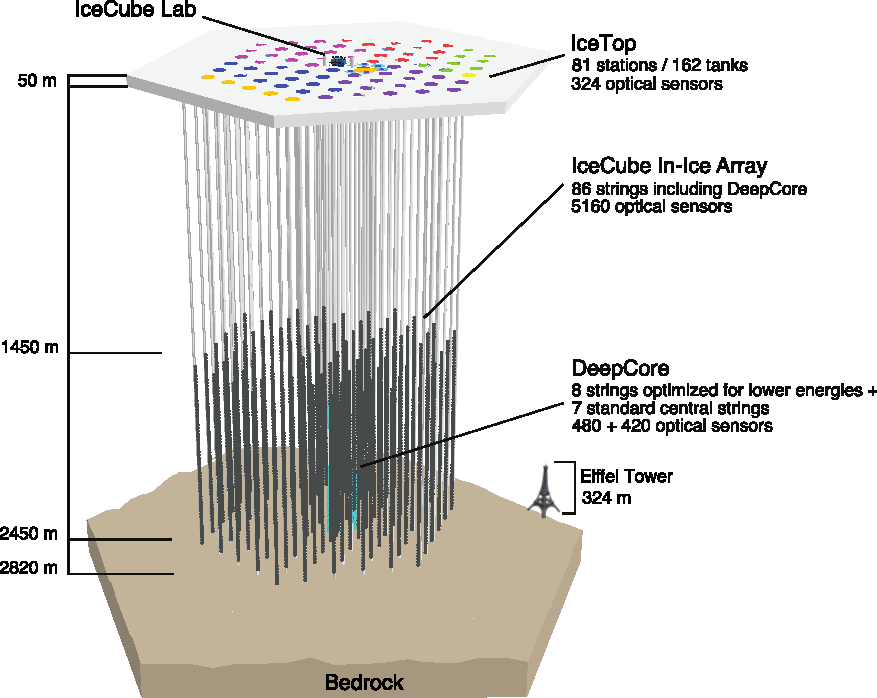
\includegraphics[width=\textwidth]{IceCubeDetector.pdf}
	\caption[Schematic view of IceCube]{\textbf{Schematic view of the IceCube Neutrino Observatory.} \cite{icecube:instrumentation} The in-ice array with the denser sub-array DeepCore as well as the surface array IceTop is sketched. Different station colors represent different deployment stages.}
	\label{icecube:detector}
\end{figure}

Neutrinos are very interesting elementary particles because of their weak interaction cross section and their electrical neutrality. This fact makes it possible for neutrinos to let them point back to their sources which is exploited in the search for astrophysical processes like active galactic nuclei, supernovae, or gamma-ray bursts. Since they are able to reach us without scattering processes, neutrinos can even give information about sources at cosmological distances. Simultaneously, the weak interaction potential is what neutrino detection makes challenging. Therefore, a detector with a large scale active volume is needed. In the case of IceCube, this is \SI{1}{\cubic\kilo\meter} of ice.

At the surface on top of the in-ice detector the cosmic ray air shower array IceTop is installed to detect Cherenkov radiation (cf. \ref{sec:cherenkov}). IceTop consists of 81 stations approximately arranged in the same grid as the in-ice strings. Each station has two tanks filled up with ice and two standard IceCube DOMs. This arrangement makes it possible for IceTop to detect primary cosmic rays (cf. \ref{sec:cosmicrays}) in the energy range of \si{\peta\electronvolt} to \si{\exa\electronvolt}. One purpose of IceTop is to provide a veto for downward-going neutrinos in the IceCube detector originating from coincident atmospheric air shower events. \cite{icecube:instrumentation} Since IceCube is investigating astrophysical neutrinos, atmospheric neutrinos are a major background.

\todo{TXS?}

\section{Cosmic Rays}\label{sec:cosmicrays}

Charged particles or nuclei that are propagating through the universe and incidentally reach the Earth's atmosphere are called cosmic rays. They were discovered by the Austrian physicist \textsc{Victor Franz Hess} in 1912 when he observed an increasing discharge of electroscopes with increasing height in seven ballon flights. \cite{cosmicrays:hess} Hess initially called this underlying radiation \enquote{durchdringende Strahlung} (\textit{penetrating radiation}).

\begin{figure}[h]
	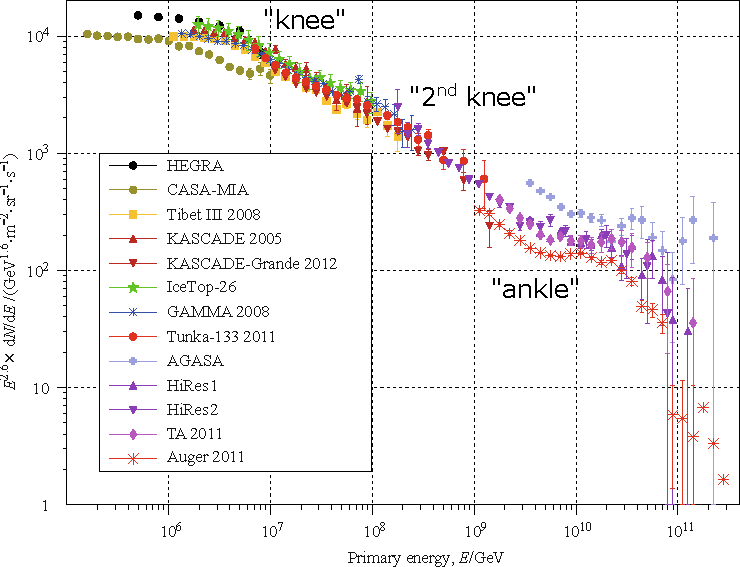
\includegraphics[width=\textwidth]{CosmicRayEnergySpectrum.pdf}
	\caption[Cosmic ray energy spectrum]{\textbf{Energy spectrum of cosmic rays measured with multiple air shower experiments.} \cite[adapted]{cosmicrays:gaisser} The three prominent regions known as \enquote{knee}, \enquote{second knee}, and \enquote{ankle} are marked. Multiplication of the spectrum by the factor $E^{2.6}$ leads to a better visibility and shows that the spectral index changes at these features.}
	\label{cosmicrays:spectrum}	
\end{figure}

When it comes to cosmic rays, ascertaining the mass composition is a key measurement for learning about their propagation in universe and about extra-galactic cosmic ray accelerators. Figure~\ref{cosmicrays:spectrum} shows that the energy spectrum of cosmic rays follows a power law:
\begin{align}
\frac{dE}{dN}\propto E^\gamma\,,
\end{align}
introducing a spectral index $\gamma$ which is dependent from the considered energy region.
Due to this interesting features, composition measurements at these \enquote{transition points} are desired in particular.

Due to the shape the spectrum is referred to as \textit{poly gonato} (Greek for \enquote{many knees}). The \enquote{knee} is assumed to be based on different rigidity\footnote{property of a magnetic field to bend a particle's trajectory} dependent cut-off energies for sub-spectra of element groups which sum up to the spectrum we observe. \cite{cosmicrays:hoerandel, cosmicrays:shapiro} At energies beyond \SI{e11}{\giga\electronvolt} a strong suppression is observed. The GZK-effect (named after Kenneth \textsc{Greisen}, Georgiy \textsc{Zatsepin}, and Vadim \textsc{Kuzmin}) is supposed to be the reason. Protons with energies above a threshold of \SI{5e19}{\electronvolt} can interact with photons of the cosmic microwave background in such a way that they produce $\pi^0$ and $\pi^+$ mesons via $\Delta^+$ resonance:
\begin{align}
\gamma_\text{CMB} + p \rightarrow \Delta^+ &\rightarrow p + \pi^0\\
&\rightarrow n + \pi^+\,.
\end{align}
Thus, the protons effectively lose about \SI{20}{\percent} of their energy. Additionally, calculations show that these interactions become quite frequent for proton energies of $E_p\gtrsim\SI{e20}{\electronvolt}$ which results in an effective cutoff of cosmic-ray energies above this region. \cite{cosmicrays:gzk}

\section{Extensive Air Showers}

If a high energetic particle -- a photon or hadron -- incidentally reaches the Earth's atmosphere, it interacts with their atoms. A common way to describe the traversed atmospheric matter for an air shower is the \textit{slant depth}
\begin{align}
X(h) = \int_{h}^{\infty}\rho(h')dh'\,
\end{align}
with the height dependent air density $\rho(h)$. Once a high energetic \enquote{primary} particle interacts with an atmospheric atom, it initiates a cascade of secondary particles. Typically, one differentiates between hadronic and electro-magnetic cascades or showers (cf. figure \ref{airshowers:cascades}). For electro-magnetic showers or sub-showers \textit{Heitler's model} is used as a simple conception. The model is based on two-body splittings of electrons, positrons, and photons by $e^+ e^-$ pair production or bremsstrahlung which occur after a fixed distance $d=\lambda_\text{em}\ln{2}$ by using the medium-specific \textit{radiation length} $\lambda_\text{em}$. In other words: after $n$ splitting processes the shower consists out of $N = 2^n = e^{x/\lambda_\text{em}}$ electrons and photons.

\begin{figure}[h]
	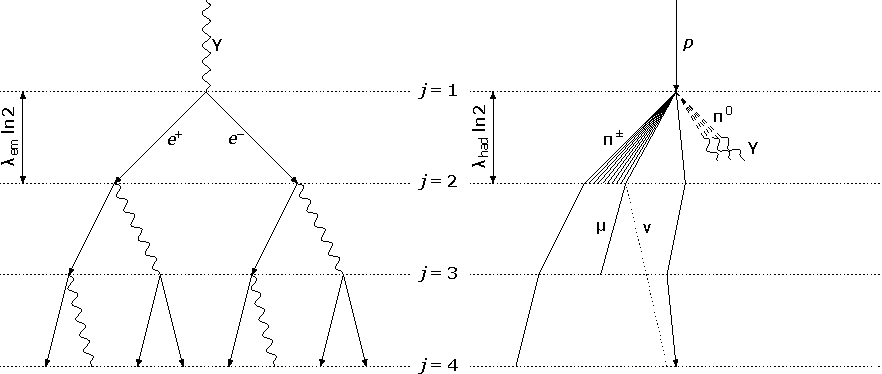
\includegraphics[width=\textwidth]{AirShowerHeitler.pdf}
	\caption[Schematic view of extensive air showers]{\textbf{Schematic view of extensive air showers.} \cite{famous:niggemann} Two possible shower formations are shown. A primary photon initiates a electro-magnetic shower (left) whereas a primary proton initiates a hadronic shower with electro-magnetic sub-showers. The splitting steps are stated as well as the interaction lengths. For the hadronic cascades not all traces are sketched for clarity reasons.}	
	\label{airshowers:cascades}
\end{figure}

The multiplication process holds, until the particle energies are high enough for pair production and bremsstrahlung. Below this energy, which Heitler named as the \textit{critical energy}~$\xi_c^e$, the shower size decreases. Hence, the maximum number of particles $N_\text{max} = 2^{n_c}$ is reached after $n_c$ splitting steps. The energy of a considered primary photon $E_\circ$ is then distributed over all secondary shower particles so that $E_\circ = \xi_c^e N_\text{max} = \xi_c^e 2^{n_c}$. With this information, one can derive the slant depth $X_\text{max}$ at which the shower has the largest size. It is
\begin{align}
	X_\text{max}^\gamma = n_c\lambda_\text{em}\ln{2} = \lambda_\text{em}\ln{\left(\frac{E_\circ}{\xi_c^e}\right)}\,.
	\label{airshowers:eq:xmax}
\end{align}
It should be mentioned that this calculation only holds for pure electro-magnetic showers which is the reason for the superscript $\gamma$ in equation \eqref{airshowers:eq:xmax}. \cite{airshowers:heitlermodel}
Since the maximum depth $X_\text{max}$ is dependent from energy and type of the primary particle it is very important for composition studies of cosmic rays. A detailed discussion on several interaction models and comparisons to simulation is done in \cite{airshowers:heitlermodel}.

\section{Detection of Air Showers via Atmospheric Cherenkov Light}\label{sec:cherenkov}

\subsection{Detection Techniques}

\begin{figure}[h]
	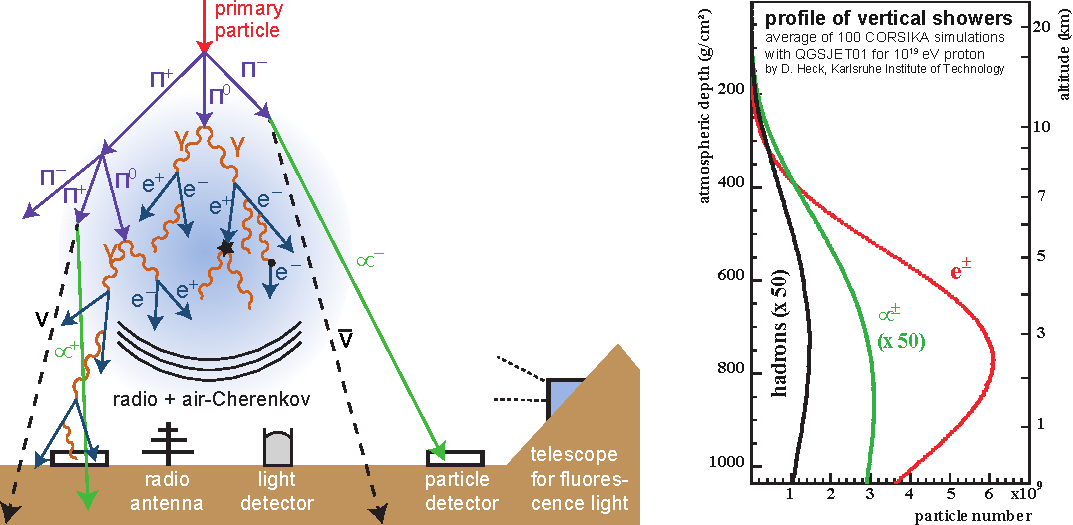
\includegraphics[width=\textwidth]{AirShowerDetection.pdf}
	\caption[Different techniques for air shower detection]{\textbf{Different techniques for the detection of atmospheric air showers.} \cite{airshowers:schroeder} }	
\end{figure}
\todo{short explanation for the different techniques}

\subsection{The Cherenkov Effect}

The Cherenkov Effect is named after the Soviet physicist \textsc(Pavel Alekseyevich Cherenkov) and describes the emission of radiation if a charged particle traverses a medium with a speed exceeding speed of light in that medium. \cite{airshowers:cherenkov} This is possible due to the fact that speed of light in a medium with a refractive index $n > 1$ is always below vacuum speed of light $c_0$ since
\begin{align}
	c = \frac{c_0}{n} \overset{n>1}{\Rightarrow} c < c_0\,.
\end{align} 
The effect is describable in two ways which are shown in figure \ref{airshowers:cherenkov}.
\begin{figure}[H]
	\centering
	\begin{subfigure}[t]{0.45\textwidth}
		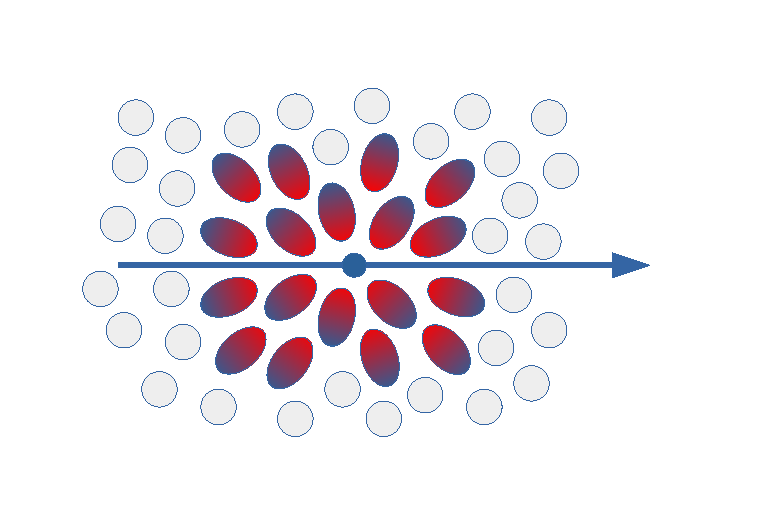
\includegraphics[width=\textwidth]{Cherenkov1Pol.pdf}
		\caption{$v < \frac{c_0}{n}$ -- The charged particle traverses the dielectric medium and polarizes its environment. For the repolarization an electric field propagates with speed of light in the medium. Since the particle's velocity is slower, no net polarization is induced and therefore no radiation is emitted.}
		\label{airshowers:cherenkov1pol}
	\end{subfigure}
	\hfill
	\begin{subfigure}[t]{0.45\textwidth}
		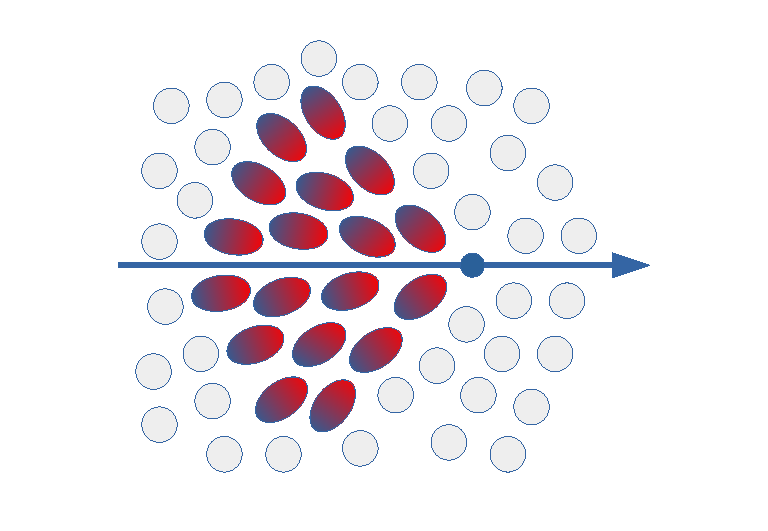
\includegraphics[width=\textwidth]{Cherenkov2Pol.pdf}
		\caption{$v > \frac{c_0}{n}$ -- The charged particles traverses the dielectric medium and polarized its environment. Since its velocity is exceeding speed of light in the medium, the electric field repolarizes the surrounding particles not fast enough so that a net polarization is induced. Cherenkov photons are emitted under a fixed angle with respect to the trajectory of the charged particle.}
		\label{airshowers:cherenkov2pol}
	\end{subfigure}
	\begin{subfigure}[t]{0.45\textwidth}
		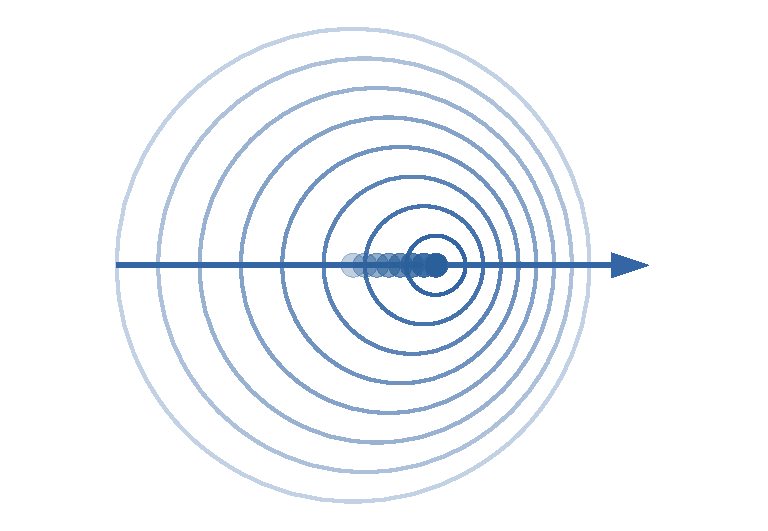
\includegraphics[width=\textwidth]{Cherenkov1Huy.pdf}
		\caption{$v < \frac{c_0}{n}$ -- The charged particle induces electro-magnetic elementary waves along its trajectory which propagate faster trough the medium than the particle. No radiation is emitted.}
		\label{airshowers:cherenkov1huy}
	\end{subfigure}
	\hfill
	\begin{subfigure}[t]{0.45\textwidth}
		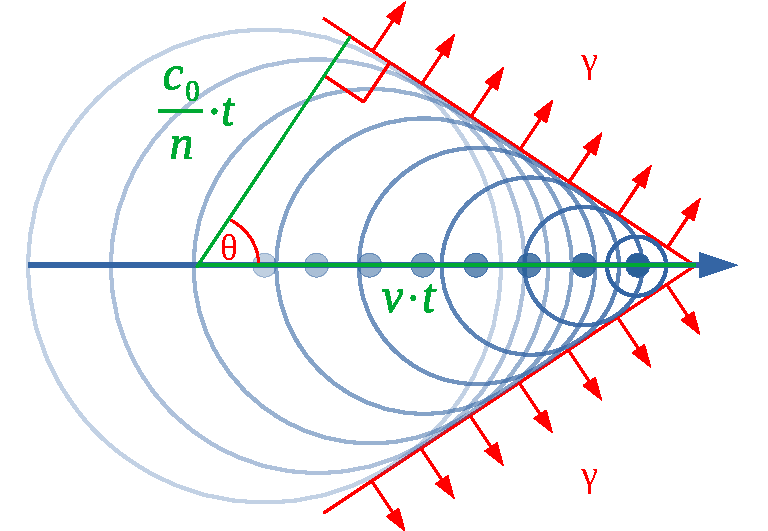
\includegraphics[width=\textwidth]{Cherenkov2Huy.pdf}
		\caption{$v > \frac{c_0}{n}$ -- The charged particle induces electro-magnetic elementary waves along its trajectory which propagate slower trough the medium than the particle. All elementary waves add up to a wavefront under a fixed angle $\theta_C$. With this model the Cherenkov effect can be interpreted as the optical analogue for the \textit{sonic boom}.}
		\label{airshowers:cherenkov2huy}
	\end{subfigure}
	\caption[Illustration for the Cherenkov effect]{\textbf{Illustration for the Cherenkov effect.} A charged particle is traversing the medium with a refractive index $n$ from left to right with velocity $v$. $c_0$ is the vacuum speed of light. In (\subref{airshowers:cherenkov1pol}) and (\subref{airshowers:cherenkov2pol}) the dipole interpretation of the Cherenkov effect is shown. (\subref{airshowers:cherenkov1huy}) and (\subref{airshowers:cherenkov2huy}) show the effect by exploiting Huygens' principle.}
	\label{airshowers:cherenkov}
\end{figure}
A \textit{Cherenkov angle} $\theta_C$ as introduced in figure \ref{airshowers:cherenkov2huy} can be calculated by applying trigonometry:
\begin{align}
	\cos{\theta_C} = \frac{c_0}{nv} = \frac{1}{n\beta}\,,
\end{align}
with the dimensionless velocity $\beta = \frac{v}{c_0}$.

Furthermore, the two Soviet physicists \textsc{Ilya M. Frank} and \textsc{Igor Y. Tamm} found a relation for the differential emission per wavelength and spatial interval known as the \textit{Frank-Tamm formula} \cite{airshowers:franktamm}:
\begin{align}
	\frac{d^2N}{dxd\lambda} = 2\pi\alpha q^2 \frac{1}{\lambda^2}\left(1-\frac{1}{n^2(\lambda)\beta^2}\right)
\end{align}
with
\begin{vardescription}
	\frac{d^2N}{dxd\lambda} & number of emitted Cherenkov photons per unit wavelength and unit propagation length\\
	\alpha & fine structure constant\\
	q & particle charge\\
	\lambda & wavelength\\
	n(\lambda) & refractive index of the medium (wavelength dependent)\\
	\beta=\frac{v}{c_0} & dimensionless relative velocity\\
\end{vardescription}
The factor $\frac{1}{\lambda^2}$ suppresses higher wavelengths so that the Cherenkov spectrum is dominant in the ultra-violet regime. Figure \ref{airshowers:cherenkovspectrum} shows a measured energy spectrum.
\begin{figure}[h]
	\centering
	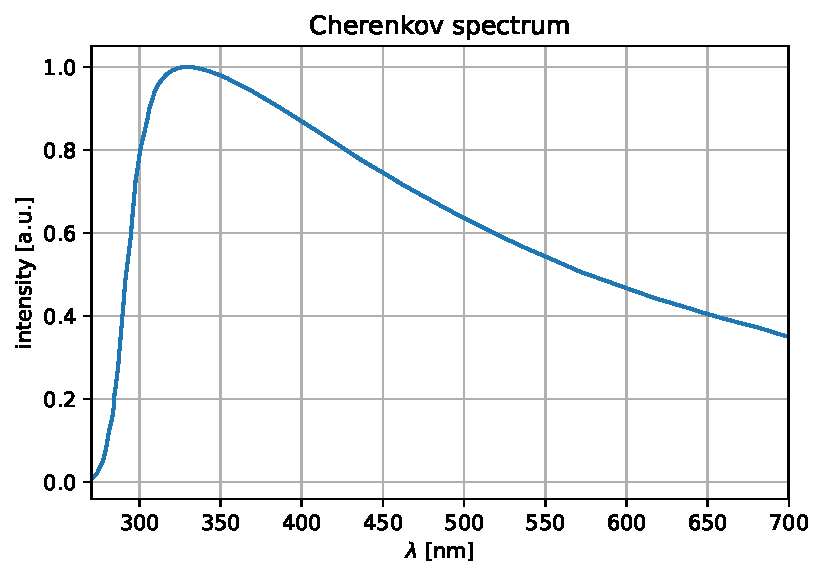
\includegraphics[width=0.5\textwidth]{CherenkovSpectrum.pdf}
	\caption[Cherenkov spectrum]{\textbf{Cherenkov wavelength spectrum.} Exemplary spectrum of Cherenkov photons measured at \SI{2200}{\meter} above sea level at the HEGRA IACT System (La Palma)\footnotemark. The falling edge towards high wavelength is proportional to $\lambda^{-2}$ whereas the falling edge towards low wavelengths is caused by atmospheric attenuation. Data adapted from \cite{airshowers:doering}.}	
	\label{airshowers:cherenkovspectrum}
\end{figure}
\footnotetext{\textbf{H}igh \textbf{E}nergy \textbf{G}amma \textbf{Ray} \textbf{A}stronomy, operated between 1987 and 2006 at Roque de los Muchachos Observatory on La Palma. \cite{airshowers:doering}}

The cone-like radiation profile of Cherenkov light with respect to the air shower axis makes it possible to reconstruct the shower direction by observing the direction of the Cherenkov photons.

\section{Imaging Air Cherenkov Telescopes}

\subsection{Imaging Technique}

\subsection{Photon Detection}

\subsection{The IceCube Air Cherenkov Telescopes IceAct}